\section{Experimental results}

We tested the methodology outlined in Section~\ref{sec:method} on the
publicly available git repositories for two popular open source
projects, the ANTLR parser generator and the Clojure language implementation.
Both are implemented in Java, and one (ANTLR) is composed of a mixture of
hand-written and automatically generated code.  

\subsection{Threshold sensitivity}
\label{sec:threshold}

The first experiment that we performed was to investigate the effect of
similarity threshold to the number of groups identified, as well as the degree
of generality present in the tree that results from all members of each group
being antiunified together. Our prediction was that at the lowest threshold
($\tau = 0.0$), when all trees are considered to be similar, their antiunification will
yield the most general pattern.  This is what was observed, in which the
antiunification result is a tree composed of a single metavariable node.
Similarly, at the highest threshold ($\tau = 1.0$), the only groupings that will be
present will be single tree sets, or sets containing identical trees for
instances of identical changes that occurred in different places.  This is
precisely what we observed, with the antiunified trees containing no 
meta-variables since antiunification of a set of identical elements is the 
element itself.

\subsection{Group counts}
\label{sec:groups}
  
We show the number of groups (broken down by type: addition, deletion, or
modification) as a function of threshold of similarity ($\tau$).
Figure~\ref{fig:clojure-number-of-modifications} shows the number of groups
for the Clojure history and Figure~\ref{fig:antlr-number-of-modifications}
shows the number of groups for the ANTLR history. In both cases, we only
consider a small portion of the full history of the VCS.

\begin{figure}
\begin{center}
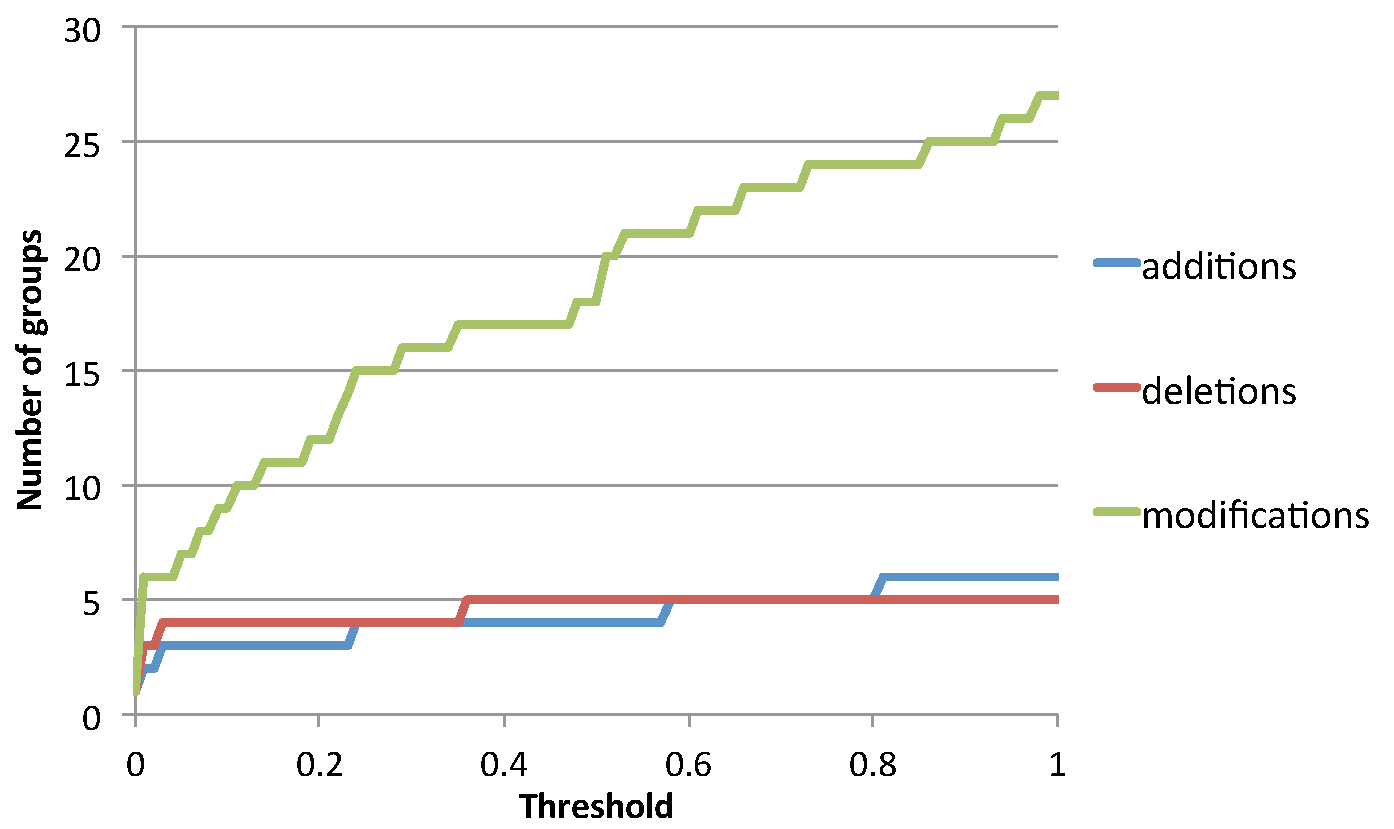
\includegraphics[width=0.44\textwidth]{figures/clojure-number-of-modifications.pdf}
\caption{Number of additions, deletions, and modifications by threshold for the Clojure source}
\label{fig:clojure-number-of-modifications}
\end{center}
\end{figure}

\begin{figure}
\begin{center}
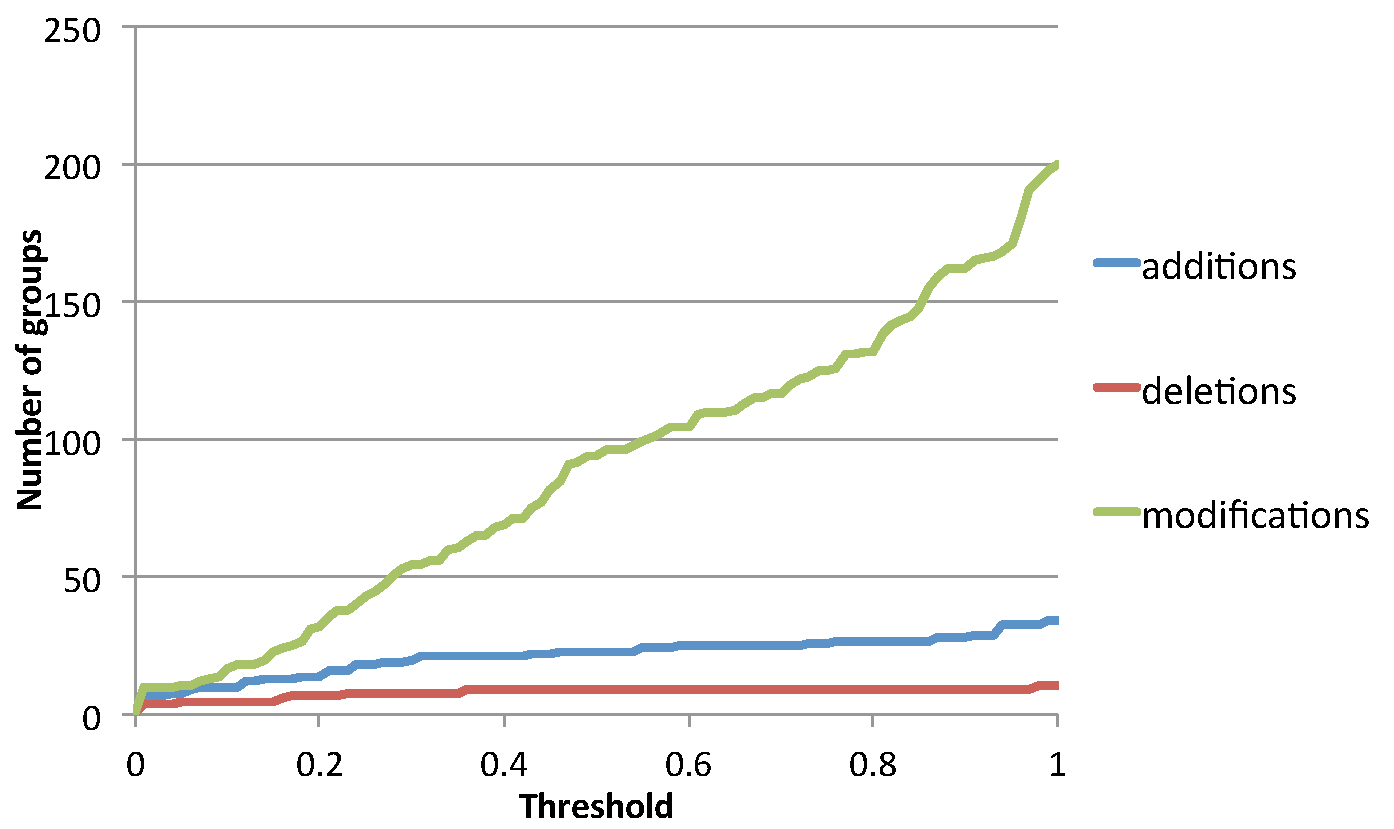
\includegraphics[width=0.44\textwidth]{figures/antlr-number-of-modifications.pdf}
\caption{Number of additions, deletions, and modifications by threshold for the ANTLR source}
\label{fig:antlr-number-of-modifications}
\end{center}
\end{figure}

At the maximum $\tau = 1.0$, the total number of changes is less than the
number of trees we started with, because some changes end up being identical.
As we can see, as $\tau$ increases, we see more groupings of changes due
to changes that were considered similar under a lower threshold being
considered dissimilar under the more restrictive threshold.  Increases in
the group count represent large groups splitting into one or more smaller groups.

As an example, at $\tau=0.15$, a single pattern for for-loops is identified:

%\newpage

\begin{java}
for ($\metavar$ = $\metavar$ ; $\metavar$ < $\metavar$ ; $\metavar$) {
    $\metavar$
}
\end{java}

As the threshold is increased to $\tau=0.25$, in addition to generic for-loops, a
cohort of changes are identified to a more specific instance of the for-loop where
the loop counter is initialized to zero:

\begin{java}
for ($\metavar$ = 0 ; $\metavar$ < $\metavar$ ; $\metavar$) {
    $\metavar$
}
\end{java}

Increasing to $\tau=0.35$, the pattern for the conditional becomes more specific
and we see what appears to be a template for using the field of an object
(e.g., {\tt args.length}) as the loop termination criterion:

\begin{java}
for ($\metavar$ = 0 ; $\metavar$ < $\metavar$.$\metavar$ ; $\metavar$) {
    $\metavar$
}
\end{java}

Similar templates emerge for code patterns such as method invocations, printing
the concatenation of two strings, and other common activities.  

%%% No time.  Save for revision if accepted.
%\jason{Talk about System.\metavar.\metavar("\metavar" + \metavar); pattern and how that evolves into
%System.out.println("\metavar" + \metavar);?}

\subsection{Pattern identification}
\label{sec:clojure}

% \subsubsection{Clojure}

Using a portion of the Clojure history, we varied $\tau$ from 0 to 1 with an
increment size of 0.01 as shown in Figure~\ref{fig:clojure-number-of-modifications}.  
Looking at just the number of deletions, we examined the
point where the number of deletions goes from 4 to 5 as the threshold changes
from 0.35 to 0.36.

The following code, presented in standard style of unified diff, shows a loop
and the lines that were removed. This example comes from a file named {\tt
PersistentArrayMap.java}:

%\jason{We should make sure none of these diffs get split over the page boundary}

\begin{java}
 public Object kvreduce(IFn f, Object init){
     for(int i=0;i < array.length;i+=2){
         init = f.invoke(init, array[i], array[i+1]);
-           if(RT.isReduced(init))
-                   return ((IDeref)init).deref();
         }
     return init;
 }
\end{java}

Given the low threshold, this deletion was considered to be similar to the
example from {\tt PersistentHashMap.java} below.
Note that whitespace in most languages is syntactically neutral and curly braces
are optional for single statement conditional or loop bodies.  As a result,
the parser used in this work gives the same AST for \verb|if (exp) { stmt; }|
and \verb|if (exp) stmt;|.   Such changes are intermingled with syntactically meaningful
changes in the unified diff format.  To clarify the specific difference that our tool 
considers to actually be different, we have added a ``>'' prefix to the appropriate lines
of the unified diff.

\begin{java}
 public Object kvreduce(IFn f, Object init){
-    for(INode node : array){
-        if(node != null){
+    for(INode node : array)
+        {
+        if(node != null)
             init = node.kvreduce(f,init);
>-                if(RT.isReduced(init))
>-                        return ((IDeref)init).deref();
-               }
-           }
+        }
     return init;
 }
\end{java}

In both cases, our tool identified for-loops where the same lines are removed.
In fact, the code for both of these is very similar perhaps owing to Java's
HashMap and ArrayMap classes being very similar in terms of interface.
Furthermore, it did this at the statement level, eg., we did not need to
consider the similarities of the file names or the method names.  The jump in
group count as $\tau$ increased corresponds to the differences in the for-loops 
that contain the change falling below the necessary threshold of
similarity for grouping.

% \subsubsection{ANTLR}

% \jason{Should we just kill this section? I feel like we should have some lesson
% learned from the antlr source, but I don't know what to pick.}

% One of the challenges with finding interesting patterns in the ANTLR source is
% that some of the files are autogenerated. We would prefer to exclude
% autogenerated files from the analysis.
